\section{Regression}

In the next three chapters, we'll look at \textbf{error-based learning}\sidenote{Error-based learning}. In general, this learning approach functions as follows:
\begin{itemize}
  \item We have a \textbf{parameterized prediction model} which is initialized with random parameters.
  \item An \textbf{error function}\sidenote{Error function} is then used to evaluate the performance of this model when it makes predictions for instances in a training dataset.
  \item Based on the results of the error function, the parameters are \textbf{iteratively adjusted} to create a more and more accurate model.
\end{itemize}

There are different approaches to realizing error-based learning:
\begin{itemize}
  \item Regression (covered in this section)
  \item SVMs (covered in the next section)
  \item Neural networks (covered in a later section)
  \item Genetic algorithms, or other evolutionary approaches
\end{itemize}

We'll start with \textbf{regression}\sidenote{Regression} and the following basic idea. 
\begin{align*}
  \text{Our model: } & f : \text{\color{mathblue}descriptive features} \rightarrow \text{\color{mathblue}target features}\\
  \text{Goal: } & \text{find } f \text{ minimizing } error(\text{\color{mathblue}prediction}, \text{\color{mathblue}observed data})
\end{align*}
When we compare this approach to decision trees, we see:
\begin{itemize}
  \item Decision trees were initially developed for categorical features and then extended to continuous features.
  \item Regression followed the reverse path, which means it's most \textbf{suitable for continuous data}.
  \item Still, both are supervised learning techniques.
\end{itemize}

\subsection{Simple linear regression}


\subsection{Multiple descriptive features}

We now assume a feature consisting of multiple elements:
\begin{align*}\begin{aligned}
  \mathbb{M}_\mathbf{w}(\mathbf{d}) &= \mathbf{w}[0] + \mathbf{w}[1]\mathbf{d}[1] + \cdots + \mathbf{w}[m]\mathbf{d}[m]\\
  &= \mathbf{w}[0] + \sum_{j=1}^m \underbrace{\mathbf{w}[j]}_{\text{weight of the }i\text{-th feature }d[j]}\mathbf{d}[j]\\
  &= \sum_{j=0}^m \mathbf{w}[j]\underbrace{\mathbf{d}[j]}_{\text{with }d[0] = 1}\\
  &= \underbrace{\mathbf{w}\cdot\mathbf{d}}_{\text{dot product of vectors}}
\end{aligned}\end{align*}

In particular, this means we have $m+1$-dimensional vectors $\mathbf{d}_i$ and $\mathbf{w}$ with $m$ as the number of features. This notational convenience extends the normal feature vector $\mathbf{d}_i'$ by $\mathbf{d}_i[0] = 1$. With $n$ instances, we therefore have the error function:
\begin{align*}\begin{aligned}
  L_2(\mathbb{M}_\mathbf{w}, \mathcal{D}) &= \frac{1}{2}\sum_{i=1}^n (t_i - \underbrace{\mathbf{w}\cdot\mathbf{d}_i}_{= \mathbb{M}_\mathbf{w}(\mathbf{d}_i)})^2
\end{aligned}\end{align*}

With our now introduced multiple descriptive feature vector, we can write down the \textbf{sketch of} the overall \textbf{algorithm} of regression:
\begin{figure}[h]
  \begin{lstlisting}[
    style=pseudocode, morekeywords={Require, if, then, else, for, each, do, make, return, repeat, until},
    caption={Sketch of regression algorithm}, captionpos=b,
    label=lst:4_regr_sketch
  ]
  Require: set of descriptive features $\mathcal{D}$
  Require: learning rate $\alpha$ (controls how quickly algorithm converges)
  Require: function $\Delta_{error}$ (determines the direction in which to adjust given weight $\mathbf{w}[i]$ to move down the slope of an error surface determined by $\mathcal{D}$)
  Require: convergence criterion (indicating when the algorithm has been completed)
  
  $\mathbf{w}\leftarrow$ random starting point in weight space // randomly pick initial point
  repeat
    for each $\mathbf{w}[j]\in \mathbf{w}$ do
      // run downhill in steepest direction with speed $\alpha$
      $\mathbf{w}[j]\leftarrow \mathbf{w}[j] + \alpha\Delta_{error}(\mathcal{D}, \mathbf{w})[j]$
  until convergence occurs // stop when improvements become too small
  \end{lstlisting}
\end{figure}

For $\Delta_{error}$ we typically choose $\frac{\delta}{\delta \mathbf{w}[j]}L_2$. This means:
\begin{itemize}
  \item If the derivative is positive, lower the weight $\mathbf{w}[j]$,
  \item If the derivative is negative, increase the weight $\mathbf{w}[j]$,
  \item While $\alpha>0$ determines the speed in both cases.
  \item Line 10 in \ref{lst:4_regr_sketch} would then result in $\mathbf{w}[j]\leftarrow \mathbf{w}[j] - \alpha \sum_{i=1}^n(t_i-\mathbf{w}\cdot\mathbf{d}_i)\mathbf{d}_i[j]$
\end{itemize}
\subsection{Interpretation of results}

For the one-feature case, the interpretation isn't difficult. We can simply see, that the target feature has some linear dependence on the descriptive feature. \begin{note} E.g., in our earlier example: the rental price has a "direct" dependency on the size.\end{note}

It becomes more difficult when \textbf{interpreting results for multiple descriptive features}. This is due to the potentially completely different ranges of those features. The weights change dramatically when the units change (e.g. when changing $cm^2$ to $m^2$). This shows that the weight itself is irrelevant, only the sign has meaning.

An alternative approach is the \textbf{significance test}\sidenote{Significance test}.

In a simple version of this, we have:
\begin{itemize}
  \item Create a regression model using $k$ descriptive features and measure the error $\Delta'$.
  \item Create $k$ regression models leaving out one descriptive feature at a time and measure the error $\Delta_i$ for $i\in[k]$.
  \item The difference in error $|\Delta' - \Delta_i|$ indicates the significance of feature $i$ for $i\in[k]$
\end{itemize}

In a more complex way (no need to know details), we follow this approach:
\begin{itemize}
  \item Null hypothesis: the feature does \textit{not} have a significant effect on the model.
  \item Null hypothesis is rejected when \textit{p-level} is too small ($1-5\%$) $\rightarrow$ a smaller p-value indicates a more important feature.
  \item In statistical hypothesis testing:
  \begin{itemize}
    \item p-value or probability value: the probability of obtaining test results at least as extreme as results actually obtained during testing
    \item Assumes a correct null hypothesis
    \item Very small p-value means: such an extreme observed outcome is very unlikely under the null hypothesis
  \end{itemize}
\end{itemize}

\subsection{Handling categorical features}

So far we assumed features (both descriptive and target) are continuous. In this chapter, we'll look at categorical descriptive and target features.
\begin{note}
  \begin{itemize}
    \item E.g., $\{$true, false$\}$, $\{$A, B, C$\}$, or similar
  \end{itemize}
\end{note}

For \textbf{categorical descriptive features}, we'll introduce $\{0$, $1\}$-features for every possible value, which is called \textbf{one hot encoding}\sidenote{One hot encoding}.
\begin{note}
  \begin{itemize}
    \item E.g., for $\{$A, B, C$\}$: A$=(1,0,0)$, B$=(0,1,0)$, C$=(0,0,1)$
  \end{itemize}
\end{note}

Next to one hot encoding, we have \textbf{single numeric value encoding}:
\begin{itemize}
  \item Binary values $\{$true, false$\}$ which can be translated to $\{$0, 1$\}$.
  \item Also, categorical variables with a clear order (ordinal) like $\{$good, average, poor$\}$ can be translated to $\{$$1.0$, $0.5$, $0.0$$\}$.
\end{itemize}

Possible issues are:
\begin{itemize}
  \item Adding order to unordered categorical variables resulting in nonsense
  \begin{note}
    \begin{itemize}
      \item E.g., simple encoding applied to country names maps numbers to countries (but no natural order exists)
    \end{itemize}
  \end{note}
  \item All encodings are approximations, so intermediate values will be considered possible by the "regression machine"
  \item One hot encoding discards dependencies
  \begin{itemize}
    \item Say if A$=1$ then logically B$=0$, but B$=0.66$ is also possible
  \end{itemize}
  \item Approach may introduce many additional features, making the problem computationally expensive
\end{itemize}

For a \textbf{categorical target feature} we can try to derive a numerical (continuous) feature. The naive approach is to find a line separating the results (try to find a line s.t. $\mathbf{w}\mathbf{d}=0$). The line then performs more of a separation than a prediction.

\begin{figure}[H]
  \centering
  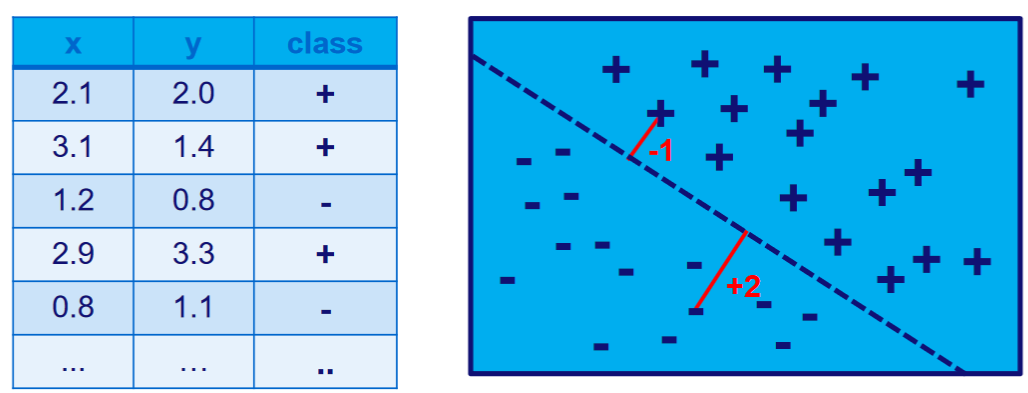
\includegraphics[width=0.6\textwidth]{assets/regression/cf__target_line.png}

  Target feature is +/- label, and not the value on the y-axis
  \caption{Seperating target feature (alternative to prediction)}
  \label{fig:4_cat_target_line}
\end{figure}

This means, we can use the $\{0, 1\}$ idea for encoding the two catgories (+/-). The model then also produces either 0 or 1:
\begin{align*}\begin{aligned}
  \mathbb{M}_\mathbf{w}(\mathbf{d})=\left\{ \begin{array}{ll}1&\text{if }\mathbf{w}\cdot\mathbf{d}\geq0\\ 0 &\text{else}\end{array} \right.
\end{aligned}\end{align*}

After this step, do business as usual e.g. by minimizing the sum of squared errors.
\begin{itemize}
  \item Notice that in this naive approach, we don't use the distance to the decision boundary yet.
  \item But this would be desirable to make the decision surface continuous or smooth and thereby more applicable to gradient descent.
\end{itemize}
\subsection{Logistic regression}
Logistic regression will help us make a 0/1-decision continuous and smooth.

First, we need the \textbf{logisitic function}\sidenote{Logistic function}:
\begin{figure}[H]
  \centering
  \begin{subfigure}{0.3\textwidth}
    \centering
    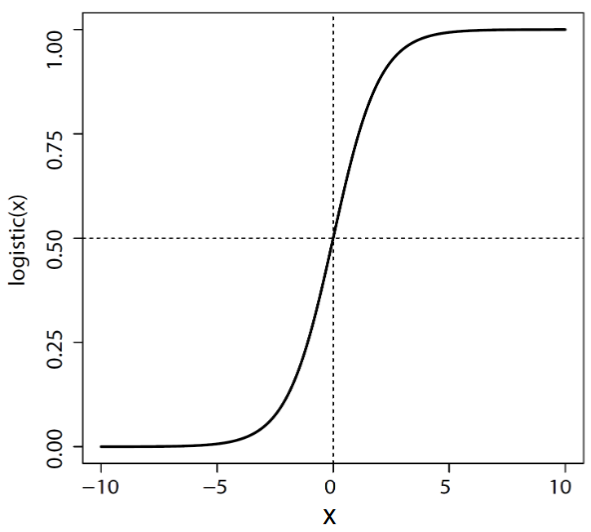
\includegraphics[width=1\textwidth]{assets/regression/lr__log_func.png}
  \end{subfigure}\hspace*{0.05\textwidth}
  \begin{subfigure}{0.6\textwidth}
    \centering
    \begin{align*}\begin{aligned}
      logistic(x) &= \frac{1}{1+e^{-x}}\\
      \frac{d}{dx}logistic(x) &= logistic(x)\cdot\big(1-logistic(x)\big)
    \end{aligned}
    \end{align*}
  \end{subfigure}
  \caption{Logistic function}
  \label{fig:4_logistic_func}
\end{figure}

\begin{itemize}
  \item Here, $e=2.7182818\cdots$ is Eulers number
  \item Any value is mapped on a value between 0 and 1
  \begin{note}\begin{itemize}
    \item $logistic(0)=0.5$, $logistic(-\infty)=0$, $logistic(+\infty)=1$
  \end{itemize}\end{note}
  \item 0 and 1 are quickly approached, therefore we can use it as a "smooth binary value"
\end{itemize}

So now, we can use \textbf{logistic regression}\sidenote{Logistic regression} instead of a hard 0/1-decision.
\begin{figure}[H]
  \centering
  \begin{subfigure}{0.4\textwidth}
    \centering
    \vspace*{0.5cm}

    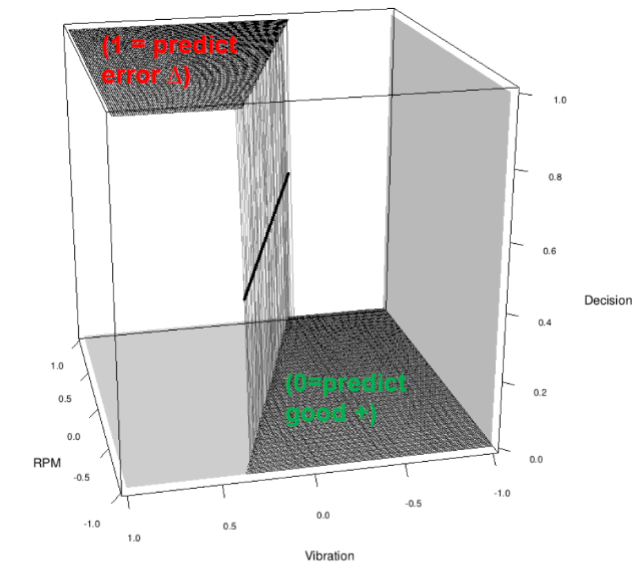
\includegraphics[width=1\textwidth]{assets/regression/lr__01.png}
    \begin{align*}
      \mathbb{M}_\mathbf{w}(\mathbf{d}) = 
        \left\{\begin{array}{ll} 
          1& \text{if }\mathbf{w}\cdot\mathbf{d}\geq0\\
          0& \text{otherwise}
        \end{array}\right.
    \end{align*}
  \end{subfigure}\hspace*{0.05\textwidth}$\rightarrow$\hspace*{0.05\textwidth}
  \begin{subfigure}{0.4\textwidth}
    \centering
    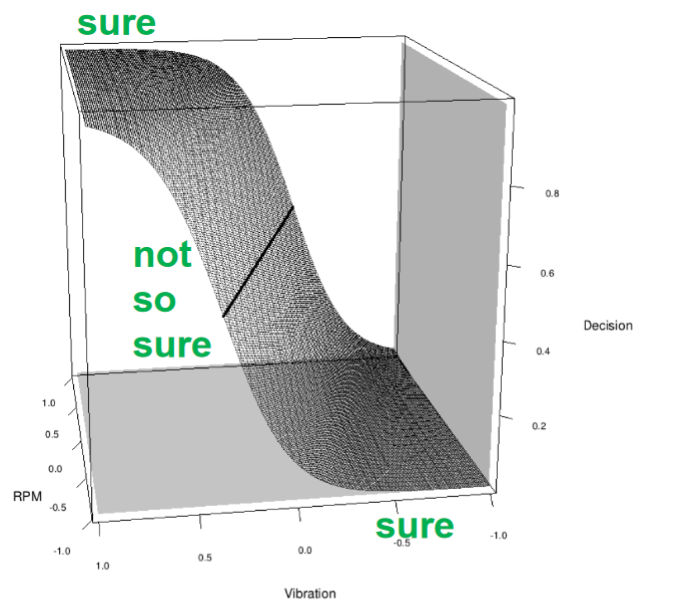
\includegraphics[width=1\textwidth]{assets/regression/lr__logistic.png}
    \begin{align*}
      \mathbb{M}_\mathbf{w}(\mathbf{d}) = logistic(\mathbf{w}\cdot\mathbf{d})
    \end{align*}
  \end{subfigure}
  \caption{Difference 0/1 and logistic}
  \label{fig:4_difference_01_logistic}
\end{figure}

The probabilistic interpretation looks as follows:
\begin{itemize}
  \item $P[t='\text{faulty}' \mid \mathbf{d}] = \mathbb{M}_\mathbf{w}(\mathbf{d})$
  \item $P[t='\text{good}' \mid \mathbf{d}] = 1 - \mathbb{M}_\mathbf{w}(\mathbf{d})$
  \item And the system is more sure about the decision, the further it is away from the separating line.
\end{itemize}

\subsection{Extensions (non-linear and multinomial)}

\textbf{Non-linear}\sidenote{Non-linear relationship} functions that can't be separated by a line can still be handled by using linear machinery. The basic idea for that is to transform the data in advance, leading to the following formula:
\begin{align*}
  \mathbb{M}_\mathbf{w}(\mathbf{d}) = \sum_{k=0}^b \mathbf{w}[k]\ \phi_k(\mathbf{d})
\end{align*}
\begin{itemize}
  \item Data in non-linear relationships is transformed \textit{before} applying the linear machinery.
  \item For that, apply "basis functions" $\phi_k$ like $\phi_0(x) = 1$, $\phi_1(x) = x$, $\phi_2(x) = x^2$, etc.
\end{itemize}

For the case of \textbf{multinomial regression}\sidenote{Multinomial regression}, we look at the problem where categorical data is not binary. As a solution for $n$ possible classes, we can split the decision into $n$ models (per class $i$ one model, classifying as "is class $i$" or "is not class $i$"). Those can then be combined back again into one model.

\begin{figure}[H]
  \centering
  \begin{subfigure}{0.7\textwidth}
    \centering
    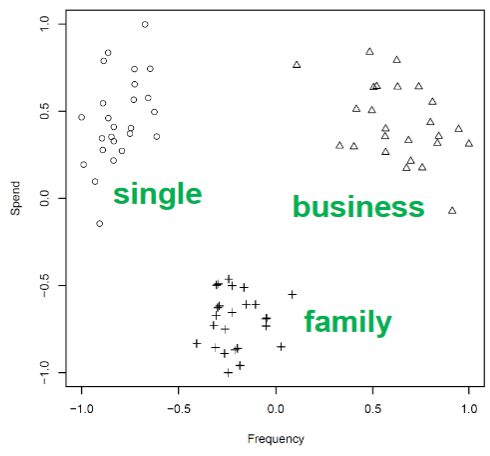
\includegraphics[width=0.4\textwidth]{assets/regression/lr__multi_problem.png}
    \subcaption{Original problem}
  \end{subfigure}
  \vspace*{0.5cm}

  \begin{subfigure}{0.7\textwidth}
    \centering
    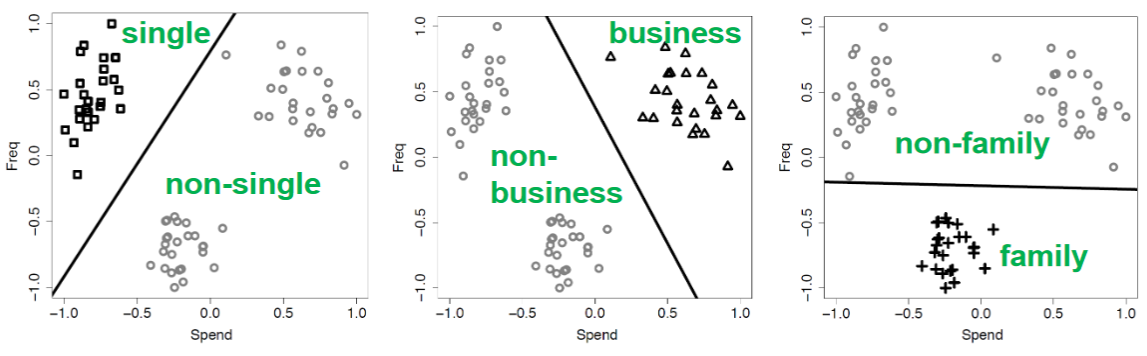
\includegraphics[width=1\textwidth]{assets/regression/lr__multi_binary.png}
    \subcaption{Binary classification}
  \end{subfigure}
  \vspace*{0.5cm}

  \begin{subfigure}{0.7\textwidth}
    \centering
    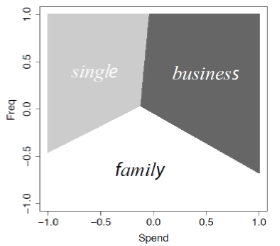
\includegraphics[width=0.4\textwidth]{assets/regression/lr__multi_sol.png}
    \subcaption{Resulting model (multinomial classification)}
  \end{subfigure}
  \caption{Combining binary (one-versus-rest) models to multinomial regression}
  \label{fig:4_multinomial}
\end{figure}

